% Created 2015-12-18 Ven 19:16
\documentclass[bigger,hyperref={colorlinks=true, urlcolor=red, plainpages=false, pdfpagelabels, bookmarksnumbered}]{beamer}
\usepackage[utf8]{inputenc}
\usepackage[T1]{fontenc}
\usepackage{fixltx2e}
\usepackage{graphicx}
\usepackage{longtable}
\usepackage{float}
\usepackage{wrapfig}
\usepackage{rotating}
\usepackage[normalem]{ulem}
\usepackage{amsmath}
\usepackage{textcomp}
\usepackage{marvosym}
\usepackage{wasysym}
\usepackage{amssymb}
\usepackage{hyperref}
\tolerance=1000
\AtBeginSection[]{\begin{frame}<beamer>\frametitle{Table of Contents}\tableofcontents[currentsection]\end{frame}}
\usepackage{listings}
\lstset{
keywordstyle=\color{blue},
commentstyle=\color{red},
stringstyle=\color{green},
basicstyle=\ttfamily\small,
columns=fullflexible,
frame=single,
basewidth={0.5em,0.4em}
}
\RequirePackage{fancyvrb}
\DefineVerbatimEnvironment{verbatim}{Verbatim}{fontsize=\small,formatcom = {\color[rgb]{0.5,0,0}}}
\usetheme{Boadilla}
\author{Stephane Genaud}
\date{\today}
\title{IMW: Middleware}
\hypersetup{
  pdfkeywords={},
  pdfsubject={},
  pdfcreator={Emacs 24.4.51.2 (Org mode 8.2.10)}}
\begin{document}

\maketitle
\begin{frame}{Outline}
\setcounter{tocdepth}{1}
\tableofcontents
\end{frame}





\section{Introduction}
\label{sec-1}
\begin{frame}[label=sec-1-1]{Technologies for Distributed Systems}
\begin{itemize}
\item Extremely fast evolution since 1985:
about a technology every 5 years.\\
\item Implementations adapt to up-to-date technology\\
     e.g If networks go faster, it is possible to convey bigger messages.\\
         If the cost of some hardware becomes low, no need to spare it.
\end{itemize}
\end{frame}

\begin{frame}[label=sec-1-2]{Technologies change but \ldots{} concepts stay}
\begin{itemize}
\item Client-server is the central concept:\\
      The \alert{client} can make a request at any time,\\
      The \alert{server} permanently waits for incoming requests
\end{itemize}
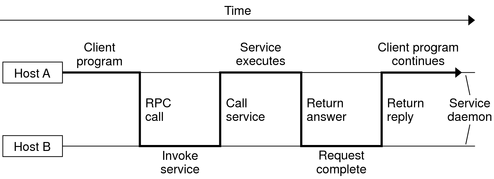
\includegraphics[width=.9\linewidth]{./img/S9_RPC_works.png}
\end{frame}

\begin{frame}[label=sec-1-3]{Middleware: definition}
\begin{block}{What is middleware?}
\begin{itemize}
\item A sofware layer between the OS and the application allowing 
a set of distributed computers to communicate in a standardized
way.
\end{itemize}
\end{block}

\begin{block}{Middleware provides inter-machines communication facilities,}
but may also include services, such as authentification services,
resource directories, distributed file catalogs, \ldots{}
\end{block}
\end{frame}

\begin{frame}[label=sec-1-4]{A Time-line of technologies}
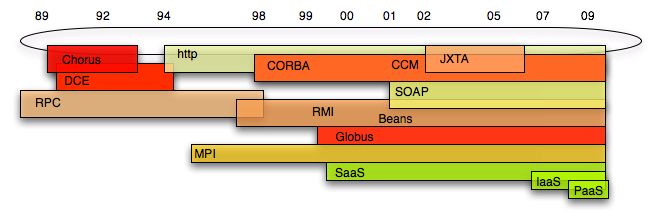
\includegraphics[width=.9\linewidth]{../img/timeline.png}
\end{frame}

\begin{frame}[label=sec-1-5]{Principle Design Choices}
\begin{itemize}
\item Abstraction vs. Performance
\item Interoperability
\item Versatility
\end{itemize}
\end{frame}
\begin{frame}[fragile,label=sec-1-6]{Abstraction}
 \begin{block}{Abstraction of communication primitives}
\begin{itemize}
\item too low level: rapidly obsolete, lower programming productivity
\item too high level: difficult to optimize for performance
\end{itemize}
\end{block}
\begin{block}{Abstraction Trade-off}
\begin{itemize}
\item independent from the architecture: execute across
different systems without \alert{source code} modification
\item Hide details related to communication/synchronization management
(e.g \texttt{Remote Procedure Calls} more abstract than \texttt{sockets})
\end{itemize}
\end{block}
\end{frame}

\begin{frame}[label=sec-1-7]{Interoperability}
\begin{block}{Machine-independent}
e.g \href{http://www.ietf.org/rfc/rfc1057.txt}{Sun RPC} 
\vspace{5mm}
\end{block}
\begin{block}{OS-independent}
e.g \href{http://www.oracle.com/technetwork/java/javase/tech/index-jsp-136424.html}{Java-RMI}
\vspace{5mm}
\end{block}
\begin{block}{Language-independent}
e.g \href{http://www.corba.org}{Corba}, \href{http://www.w3.org/TR/soap/}{SOAP}
\end{block}
\end{frame}
\begin{frame}[label=sec-1-8]{Versatility}
The more general, the more versatile 
\begin{itemize}
\item Example 1: SOAP communicates through XML pieces of text
\item $\Rightarrow$ SOAP toolkits can be found for almost all languages.
\end{itemize}
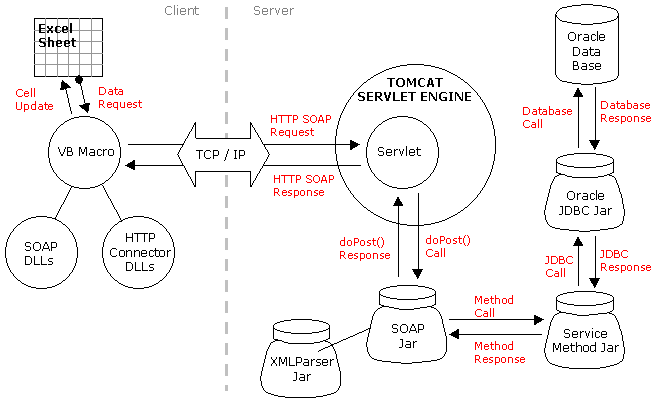
\includegraphics[width=.9\linewidth]{../soap-img/soapuser-archi1.png}
\end{frame}

\section{Sun RPC}
\label{sec-2}
\begin{frame}[label=sec-2-1]{Background}
Sun RPC  (aka RPC ONC (Open Network Computing)) 
\begin{itemize}
\item are the original RPC (\href{http://tools.ietf.org/html/rfc1831}{RFC 1831}), introduced by Sun in 1988
\item motivation: provide a support to inter-machines services
\item NFS as first target, NIS, \ldots{}.
\item is open source software (BSD license since 2009)
\end{itemize}
\end{frame}
\begin{frame}[label=sec-2-2]{Interoperability}
\begin{itemize}
\item ONC RPC allow programs on different OS and machines to communicate
\item It may be in different languages but C in 99\% cases.
\item Relies on \href{http://www.ietf.org/rfc/rfc4506.txt}{XDR} (eXternal Data Representation)
\end{itemize}
\end{frame}

\begin{frame}[fragile,label=sec-2-3]{RPC service identification}
 \begin{block}{Services are identified by}
\begin{enumerate}
\item the program name (\verb~prog_name~)
\item the program version (\verb~prog_ver~)
\item the function name
\end{enumerate}
\end{block}
\begin{beamercolorbox}{Example}
\lstset{language=C,label= ,caption= ,numbers=none}
\begin{lstlisting}
  program MYPROG {
    version VERSION_ONE {
      void MYPROG_NULL(void) = 0;
      answer MYPROG_MYFUNC(data) = 1;
    } = 1;
  } = 0x2000:0001;
\end{lstlisting}
\end{beamercolorbox}
\end{frame}

\begin{frame}[fragile,label=sec-2-4]{Service Registration (portmap)}
 This service must be registered in a directory service generally called \emph{portmapper} 
\begin{itemize}
\item acts as a name server
\item converts : <prog$_{\text{name}}$ + ver + protocol> to <portnumber>
\item exact service name depending on sytem/distribution : \texttt{rpcbind} (or sometimes \texttt{portmap}, or \texttt{rpc.portmap})
\item attached to port 111
\end{itemize}
\end{frame}

\begin{frame}[fragile,label=sec-2-5]{Service Registration (prognum)}
 Registration needs (\texttt{rpcregister} 1st arg for example)
a 32-bit identifier (sometimes called RPC port) 

\begin{center}
\begin{tabular}{ll}
Range (hex.) & role\\
\hline
00000000-1fffffff & defined by rpc@sun.com\\
20000000-3fffffff & defined by user\\
40000000-5fffffff & transient (dynamic server)\\
60000000-ffffffff & reserved\\
\end{tabular}
\end{center}
\end{frame}


\begin{frame}[fragile,label=sec-2-6]{Standard RPC services}
 \begin{block}{file \texttt{/etc/rpc}}
\lstset{language=C,label= ,caption= ,numbers=none}
\begin{lstlisting}
portmapper  100000  
rstatd      100001  
rusersd     100002  
nfs         100003  
ypserv      100004 
mountd      100005 
ypbind      100007
walld       100008
\end{lstlisting}
\end{block}

\begin{block}{Tips \& Tricks : rpc services \emph{may not} be started on recent systems}
\begin{itemize}
\item MacOSX since Mavericks : run \texttt{sudo launchctl start com.apple.rpcbind}
\item Linux : check that package \texttt{rpcbind} is installed
\end{itemize}
\end{block}
\end{frame}


  \#+begin$_{\text{src}}$ c
  \% rpcinfo -p
    program vers proto   port
   100000    2   tcp    111  portmapper
   100000    2   udp    111  portmapper
536870913    1   udp  58764
536870913    1   tcp  65106
  \#+end$_{\text{src}}$ c
Two last lines are one user program.





\begin{frame}[fragile,label=sec-2-8]{Programming with ONC RPC}
 Two layers:
\begin{block}{The \alert{higher} layer: small set of functions to describe and call services in a simple way.}
\begin{itemize}
\item Essential primitives: \texttt{registerrpc()} and \texttt{callrpc()} \\
\item However, limitations: udp only, no auth, and encoding/decoding by hand.
\end{itemize}
\end{block}

\begin{block}{The \alert{lower} layer: 20+ functions to fine tune the calls.}
\begin{itemize}
\item Much more complex, used for stressed services, for example 
to implement asynchronous RPC and authentification.
\end{itemize}
\end{block}
\end{frame}

\begin{frame}[fragile,label=sec-2-9]{Server-side steps}
 The server must \alert{register}: asks the local portmap to:
\begin{enumerate}
\item create a new entry so that clients can be routed
\item associate a service number and the address of the function 
that implements it, or the address of the \emph{dispatcher}.
\end{enumerate}
\begin{block}{The primtives are}
\begin{itemize}
\item \texttt{svc\_register()} and \texttt{pmap\_set()} (low level)
\item \texttt{rpcregister()} (high level)
\item on exit, \texttt{svc\_unregister()}, \texttt{pmap\_uset()}
\end{itemize}
\end{block}
\end{frame}
\begin{frame}[fragile,label=sec-2-10]{Client-side steps}
 The client must initialize (1), lookup in remote portmap to find the service (2),
then, several calls can be made afterwards (3):
\begin{enumerate}
\item \texttt{clnt\_create()} / \texttt{clnttcp\_create()} / \texttt{clntudp\_create()},
\item \texttt{pmap\_getport()}
\item \texttt{clnt\_call()}
\end{enumerate}

The higher level \texttt{callrpc()} does steps 1, 2 and 3 in a row.
\end{frame}

\begin{frame}[fragile,label=sec-2-11]{Example of high-layer usage (server side 1/2)}
 \emph{Define the service on the server:}
\lstset{language=C,label= ,caption= ,numbers=none}
\begin{lstlisting}
#include <rpc/xdr.h>
#include <rpc/rpc.h>

int* my_function(int *n) {
   static int res;
   *n = *n + 1;
   res= *n; 
   return (&res);
}
\end{lstlisting}
\end{frame}

\begin{frame}[fragile,label=sec-2-12]{Example of high-layer usage (server side 2/2)}
 \emph{Register the service on the server:}
\lstset{language=C,label= ,caption= ,numbers=none}
\begin{lstlisting}
#define PROGNUM 0x20000100                                                      
#define VERSNUM 1                                                               
#define PROCNUM 1

int main (void) {
   registerrpc( PROGNUM,
                VERSNUM,
                PROCNUM,
                my_function, /*ptr to function*/
                (xdrproc_t) xdr_int, /*encode input*/
                (xdrproc_t) xdr_int);/*decode output*/

    svc_run(); /*  server starts listening ... */
}
\end{lstlisting}
\end{frame}

\begin{frame}[fragile,label=sec-2-13]{Example of high-layer usage (client side 1/2)}
 \emph{Call the service from the client:}
\lstset{language=C,label= ,caption= ,numbers=none}
\begin{lstlisting}
int main (int argc, char **argv) {
 int n=0x41424344;
 char *host = argv[1];
 int stat;
 stat = callrpc(host,
                PROGNUM,
                VERSNUM,
                PROCNUM,
                (xdrproc_t) xdr_int,  //intput encoding
                (char *) &n,          //input param
                (xdrproc_t) xdr_int,  //output decoding
                (char *) &res);       //return of func
}
\end{lstlisting}
\end{frame}


\begin{frame}[fragile,label=sec-2-14]{Try It}
 \begin{itemize}
\item Sources : \href{http://icps.u-strasbg.fr/~genaud/courses/sd/src/rpc/example_1.tar.gz}{Example 1}
\end{itemize}

\begin{block}{Have you noticed?}
\begin{itemize}
\item There are only \alert{1} parameter for input and \alert{1} for output
\item the variable returned \texttt{res} is declared \texttt{static} because it may have to survive for a while
\end{itemize}
\end{block}
\end{frame}


\begin{frame}[fragile,label=sec-2-15]{Another way: \texttt{rpcgen}}
 \begin{itemize}
\item Taking care of conversion through XDR is difficult
\item The \texttt{rpcgen} compiler automates the process of writing RPC applications
\item \texttt{rpcgen} accepts interface descriptions in \href{http://docs.oracle.com/cd/E19683-01/816-1435/6m7rrfn9k/index.html}{RPCL (RPC Language)}
\item and generates skeletons programs (C code)
\end{itemize}
\end{frame}

\begin{frame}[fragile,label=sec-2-16]{Example with \texttt{rpcgen}}
 \begin{itemize}
\item Consider an \emph{operation} \texttt{addition}, that adds up 2 \texttt{int} s
\item Describe this service in a file \texttt{myservice.x}
\end{itemize}
\lstset{language=C,label= ,caption= ,numbers=none}
\begin{lstlisting}
struct data {
  int arg1;  int arg2;
};
typedef struct data data;
struct response {
  int result; unsigned char error;
};
typedef struct response response;

program MYCOMPUTATION {
  version VERSION_ONE{
    void MYCOMPUTATION_NULL(void) = 0;
    response MYCOMPUTATION_ADDITION(data) = 1;
  } = 1;
} = 0x20000001;
\end{lstlisting}
\end{frame}

\begin{frame}[fragile,label=sec-2-17]{Files generated by \texttt{rpcgen}}
 \begin{itemize}
\item Generate the skeletons
\end{itemize}
\lstset{language=C,label= ,caption= ,numbers=none}
\begin{lstlisting}
   % rpcgen -a myservice.x
\end{lstlisting}
\begin{itemize}
\item The following files are generated
\end{itemize}
\lstset{language=C,label= ,caption= ,numbers=none}
\begin{lstlisting}
  myservice.h        /* parameter definitions */
  myservice_xdr.c    /* XDR conversion */
  myservice_svc.c    /* stubs server */   
  myservice_clnt.c   /* stubs client */
  myservice_server.c /* server code */
  myservice_client.c /* client code */
\end{lstlisting}
\begin{itemize}
\item Only the \texttt{\_client.c} and \texttt{\_server.c} files are intended to the programmer
\end{itemize}
\end{frame}

\begin{frame}[label=sec-2-18]{Try It (client/server with rpcgen)}
\begin{itemize}
\item Here are skeletons for a basic client / server scheme
\item Sources : \href{http://icps.u-strasbg.fr/~genaud/courses/sd/src/rpc/example_2_rpcgen_incomplete.tar.gz}{Example 2}
\end{itemize}
\end{frame}

\begin{frame}[fragile,label=sec-2-19]{Code Generated by \texttt{rpcgen}}
 \begin{itemize}
\item In \texttt{\_client.c}, examples calls:
\end{itemize}
\lstset{language=C,label= ,caption= ,numbers=none}
\begin{lstlisting}
   result = mycomputation_addition_1(
              &mycomputation_addition_1_arg, clnt);
   if (result == NULL) {
        clnt_perror(clnt, "call failed:");
    }
\end{lstlisting}

\begin{itemize}
\item In \texttt{\_server.c}, \emph{handlers} are created
\end{itemize}
\lstset{language=C,label= ,caption= ,numbers=none}
\begin{lstlisting}
response *
mycomputation_addition_1_svc(data *argp,
                             struct svc_req *rqstp)
{
      static response  result;
      /* insert server code here */
      return(&result);
}
\end{lstlisting}
\end{frame}

\begin{frame}[fragile,label=sec-2-20]{RPCL in Brief (enumeration, constants \& simple)}
 \begin{block}{Enumerations and Constants}
\lstset{language=C,label= ,caption= ,numbers=none}
\begin{lstlisting}
enum colortype { RED = 0, GREEN = 1,BLUE = 2  };
const PI = 3.14;
\end{lstlisting}
\end{block}
\begin{block}{Simple Declarations}
\lstset{language=C,label= ,caption= ,numbers=none}
\begin{lstlisting}
int length;
colortype c;
\end{lstlisting}
\end{block}
\begin{block}{Added types (bool and string)}
\begin{itemize}
\item \texttt{bool} : boolean, can take TRUE or FALSE values
\item \texttt{string}: translated to \texttt{char *} (See variable length array).
\end{itemize}
\end{block}
\end{frame}
\begin{frame}[fragile,label=sec-2-21]{RPCL in Brief (arrays)}
 \begin{block}{Fixed-length arrays}
\lstset{language=C,label= ,caption= ,numbers=none}
\begin{lstlisting}
int length[5];
color palette[8];
\end{lstlisting}
\end{block}

\begin{block}{Variable-length arrays}
\begin{itemize}
\item The maximum size is specified between angle brackets, or may be ommitted:
\end{itemize}
\lstset{language=C,label= ,caption= ,numbers=none}
\begin{lstlisting}
int notes_serie<20>;   # at most 20
int heights<>;         # unlimited
string message<256>;
\end{lstlisting}
each will translate to a C struct, e.g:
\lstset{language=C,label= ,caption= ,numbers=none}
\begin{lstlisting}
struct {
   u_int heights_len;/* # of items in array */
   int *heights_val; /* pointer to array */
} heights;
\end{lstlisting}
\end{block}
\end{frame}
\begin{frame}[fragile,label=sec-2-22]{RPCL in brief (typedef)}
 \begin{block}{Type definitions}
Same syntax as C typedef
\lstset{language=C,label= ,caption= ,numbers=none}
\begin{lstlisting}
typedef string name_t<255>; 
typedef string longstring<>;
\end{lstlisting}
will be translated into C code:
\lstset{language=C,label= ,caption= ,numbers=none}
\begin{lstlisting}
typedef char *name_t;
typedef char *longstring;
\end{lstlisting}
\end{block}
\end{frame}

\begin{frame}[fragile,label=sec-2-23]{RPCL in Brief (pointers)}
 \begin{itemize}
\item Pointer declarations are as in C. Address pointers are not sent over the network. 
Instead, data pointed to are copied. This is useful for sending recursive data 
types such as lists and trees.
\end{itemize}
\lstset{language=C,label= ,caption= ,numbers=none}
\begin{lstlisting}
 tree_t *t;
\end{lstlisting}
\end{frame}
\begin{frame}[fragile,label=sec-2-24]{RPCL in Brief (struct)}
 \begin{itemize}
\item Translates as is in C, excepted that an extra typedef is generated.
\end{itemize}
\lstset{language=C,label= ,caption= ,numbers=none}
\begin{lstlisting}
struct coord {  int x;  int y;  };
\end{lstlisting}
Translates to:
\lstset{language=C,label= ,caption= ,numbers=none}
\begin{lstlisting}
struct coord {  int x;  int y;  };
typedef struct coord coord;
\end{lstlisting}
which allows to use \texttt{coord} instead of \texttt{struct coord}
\end{frame}



\begin{frame}[fragile,label=sec-2-25]{Tips \& Tricks}
 \begin{block}{Linux}
\begin{itemize}
\item Install: rpc lib provided by package  \texttt{libtirpc-dev}  (0.2.2-5 on ubuntu 12.04)
\item Run: a portmapper is provided by package \texttt{rpcbind}
\item Run: \texttt{svc\_register()} might refuse to register ("credentials problem") 
$\Rightarrow$ Start server as root or in sudo mode.
\item Initialize array variables before calling remote functions 
("Can't encode arguments" error).
\end{itemize}
\end{block}
\begin{block}{MacOSX}
\begin{itemize}
\item Install: the 'Command line tools' element from Xcode in the distrib
or download it fom  \href{https://developer.apple.com/downloads/}{Apple} .
\item Use: \texttt{rpcgen -C} to force generation of ANSI-C code
\end{itemize}
\end{block}
\end{frame}

\section{Java RMI}
\label{sec-3}
\begin{frame}[fragile,label=sec-3-1]{History}
 \begin{itemize}
\item Created by Sun in 1998
\item Java only
\item Available since JDK >= 1.1
\item Since JDK 1.5, stubs are automatically generated (no \texttt{rmic})
\end{itemize}
\end{frame}
\begin{frame}[fragile,label=sec-3-2]{RPC in the world of RMI}
 \begin{itemize}
\item RMI provides access to \alert{objects} and their \alert{methods}
\item In contrast to Sun RPC, not only data can be passed
to remote computations, but also objects that can contain
code and data.\\[5mm]

\item There are 2 ways to communicate in this object-oriented
paradigm: 
\begin{enumerate}
\item through the \texttt{Remote} class
\item through the \texttt{Serializable} class
\end{enumerate}
\end{itemize}
\end{frame}

\begin{frame}[label=sec-3-3]{The Remote class}
definition: An object of the Remote class can be used remotely.
It can be used:
\begin{itemize}
\item in the address space of the JVM that created it,
\item in the address spaces of other JVMs through \emph{handles} (aka \emph{proxies}).
\end{itemize}

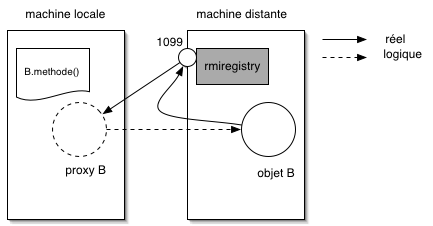
\includegraphics[width=.9\linewidth]{../img/proxy.png}
The call to a remote object's method is exactly (syntactically) the same as a local one.   
\end{frame}

\begin{frame}[fragile,label=sec-3-4]{The Remote class  and interface}
 \begin{block}{A Remote class must be defined in 2 parts}
\begin{itemize}
\item an interface (shared between client and server)
\item the class itself (implem. on client)
\end{itemize}
\end{block}
\begin{block}{Interface}
\lstset{language=java,label= ,caption= ,numbers=none}
\begin{lstlisting}
    public interface MyExample extends Remote {...}
\end{lstlisting}
\end{block}

\begin{block}{Class}
\lstset{language=java,label= ,caption= ,numbers=none}
\begin{lstlisting}
public class MyExampleImpl 
  extends    UnicastRemoteObject
  implements MyExample  {
    ...
   }
\end{lstlisting}
\end{block}
\end{frame}

\begin{frame}[label=sec-3-5]{The Serializable class}
definition: an object of the class Serializable is an object
that can be copied from one address space to another.
\end{frame}

\begin{frame}[fragile,label=sec-3-6]{Registering the services}
 A process called \alert{rmiregistry} is in charge of service registration\\
   (Equivalent of portmapper)
\begin{block}{Characteristics of \texttt{rmiregistry}}
\begin{itemize}
\item runs on the same host as the services
\item default port is 1099
\item can be started by program
\end{itemize}
\end{block}
\end{frame}

\begin{frame}[label=sec-3-7]{Example 1: Remote object with primitive types}
Example parameter passing using primitive types (e.g. int, float, ..) or arrays (e.g. String) 
\begin{itemize}
\item In general, parameters just need to be \alert{serializable} (java.io.Serializable).
\end{itemize}
\begin{block}{The different pieces of code}
\begin{itemize}
\item The service: description of the function prototype
\item The service: the implementation of the service
\item The server: a generic code which registers the service
\item The client: the code that uses the service
\end{itemize}
\end{block}
\end{frame}

\begin{frame}[fragile,label=sec-3-8]{Example 1: Service Description}
 A service is described by an \alert{interface}.
\begin{itemize}
\item known by the client and the server.
\end{itemize}

\lstset{language=java,label= ,caption= ,numbers=none}
\begin{lstlisting}
import java.rmi.Remote;
import java.rmi.RemoteException;

public interface Operation extends Remote {

    public int addition(int a, int b) 
                    throws RemoteException ;
}
\end{lstlisting}
\end{frame}

\begin{frame}[fragile,label=sec-3-9]{Example 1: Service Implementation}
 \begin{itemize}
\item Only the server \alert{implements} the service.
\end{itemize}
\lstset{language=java,label= ,caption= ,numbers=none}
\begin{lstlisting}
import java.rmi.server.UnicastRemoteObject ;
import java.rmi.RemoteException ;
import java.net.InetAddress.* ;
import java.net.* ;

public class OperationImpl extends UnicastRemoteObject
  implements Operation  {

    public OperationImpl () throws RemoteException {
        super();
    };

    public int addition(int a, int b) 
                    throws RemoteException {
      return( a + b) ;
  }
}
\end{lstlisting}
\end{frame}

\begin{frame}[fragile,label=sec-3-10]{Example 1: Service Registration}
 \begin{itemize}
\item The first server task is to register the service 
in the rmiregistry under a name (here \emph{Operation})
\end{itemize}

\lstset{language=java,label= ,caption= ,numbers=none}
\begin{lstlisting}
public class Serveur {
  public static void main(String [] args) {
    try {
       OperationImpl une_op = new OperationImpl ();
       Naming.rebind("rmi://localhost/Operation",une_op) ;
       System.out.println("Serveur pret");
     }
     catch (Exception e) { 
           System.out.println(re) ; 
     }
}
\end{lstlisting}
\end{frame}

\begin{frame}[fragile,label=sec-3-11]{Example 1: Client code}
 \begin{itemize}
\item gets a reference to the service in the registry (proxy)
\item call the service using that reference
\end{itemize}

\lstset{language=java,label= ,caption= ,numbers=none}
\begin{lstlisting}
import java.rmi.* ;
import java.net.MalformedURLException ;
import java.io.*;

public class Client {
  public static void main(String [] args) {
    try {
         Operation o = (Operation) 
             Naming.lookup("//"+args[0]+"/Operation");
         System.out.println("Client: 33+45= ?");
         int r = o.addition( 33, 45 );
         System.out.println("33+45="+ r );
     }
     catch (Exception e) { System.out.println(e) ; }
   }
}
\end{lstlisting}
\end{frame}

\begin{frame}[fragile,label=sec-3-12]{Try It (RMI basic client/server)}
 \begin{itemize}
\item Here are the source code for Example 1
\item Sources : \href{http://icps.u-strasbg.fr/people/genaud/public_html/courses/sd/src/rmi/rmi_base_example_add.tar.gz}{Example 1 (base$_{\text{example}}$$_{\text{add}}$)}
\item Choose either \texttt{Serveur\_version\_Naming.java} or \texttt{Serveur\_version\_Locateregistry.java}
\end{itemize}
\end{frame}

\begin{frame}[fragile,label=sec-3-13]{Trouble shooting 1}
 \begin{block}{Observation}
\texttt{connection refused} error when contacting the server.
\end{block}
\begin{block}{Why?}
\texttt{\$JAVA\_HOME/lib/security/java.policy} too restrictive 
\end{block}
\begin{block}{Solution}
Override standard permissions: 
\texttt{java -Djava.security.policy=myperm Server}
whith file \texttt{myperm}:

\lstset{language=java,label= ,caption= ,numbers=none}
\begin{lstlisting}
grant {
    permission java.net.SocketPermission
    "*:80-65535","connect,accept,listen,resolve";
    permission java.security.AllPermission;
};
\end{lstlisting}
\end{block}
\end{frame}

\begin{frame}[fragile,label=sec-3-14]{Trouble shooting 2}
 \begin{block}{Observation}
When calling the RPC (hence after the lookup), the client ends with:
\texttt{java.rmi.ConnectException: Connection refused to host: 127.0.0.1}
\end{block}

\begin{block}{Why?}
In some linux distributions, the name resolution for hostname
takes 127.0.0.1 from \texttt{/etc/hosts} instead of public IP.
\end{block}

\begin{block}{Solution}
run the server by overriding its IP
\lstset{language=java,label= ,caption= ,numbers=none}
\begin{lstlisting}
    java -Djava.rmi.server.hostname=<my ip here> Server
\end{lstlisting}
\end{block}
\end{frame}

\begin{frame}[fragile,label=sec-3-15]{Trouble shooting 3}
 \begin{block}{Debugging}
In case your server-side implementation crashes due to a programming error,
you may experience errors when accessing the remote objects.
\end{block}

\begin{block}{Solution}
To better spot the error, run the server with logging on:
\lstset{language=java,label= ,caption= ,numbers=none}
\begin{lstlisting}
    java -Djava.rmi.server.logCalls=true Server
\end{lstlisting}
(add -Djava.security.policy= \ldots{} if needed) 
\end{block}
\end{frame}
\section{Corba}
\label{sec-4}
\begin{frame}[label=sec-4-1]{History}
\begin{block}{Context}
\begin{itemize}
\item A specification defined by the \emph{Object Management Group} (OMG), 
composed of about 1000 members
\item currently CORBA 3.0
\item Implementors then propose implementations
\end{itemize}
\end{block}

\begin{block}{Implemenations}
Commercial :
\begin{itemize}
\item ORBIS, IONA, VisiBroker, ORBacus, \ldots{}.
\end{itemize}
Open source:
\begin{itemize}
\item JDK, MICO, JacORB, TAO, \ldots{}
\end{itemize}
\end{block}
\end{frame}

\begin{frame}[fragile,label=sec-4-2]{Sun Implementation}
 \begin{block}{Since 1.3}
\begin{itemize}
\item JDK provides IDL-to-Java compiler \texttt{idlj}
\end{itemize}
\end{block}
\begin{block}{Since 1.4}
\begin{itemize}
\item includes support for the Portable Object Adapter (POA)
\item an Object Request Broker Daemon (ORBD) to locate/invoke persistent objects.
\item \texttt{servertool}  command line to (un)register/startup/shutdown a persistent server
\end{itemize}
\end{block}

\begin{block}{Imports}
\lstset{language=java,label= ,caption= ,numbers=none}
\begin{lstlisting}
import org.omg.CosNaming.*;
import org.omg.CosNaming.NamingContextPackage.*;
import org.omg.CORBA.*;
\end{lstlisting}
\end{block}
\end{frame}

\begin{frame}[label=sec-4-3]{Characteristics}
CORBA = Common Object Request Broker Architecture

\begin{block}{A RPC framework}
\begin{itemize}
\item object oriented
\item multiple-OS, multiple languages can be involved
\item analogy of the "software bus"
\end{itemize}
\end{block}
\begin{block}{External Services}
\begin{itemize}
\item helper services, can connect to the bus
\item services: naming, transaction, persistence \ldots{}
\end{itemize}
\end{block}
\end{frame}

\begin{frame}[label=sec-4-4]{IDL}
The Interface Definition Language:
equivalent to the RPC Language.

\begin{itemize}
\item defines the \alert{methods} a server proposes
\item defines the \alert{data} that can be accessed from the client (get/set)
\end{itemize}

From IDL, generation of concrete code to
represent data and methods in the chosen language.
\end{frame}

\begin{frame}[fragile,label=sec-4-5]{IDL structure}
 Three hierarchical elements:
\begin{enumerate}
\item \texttt{Module} : namespaces (correspond to Java packages)
\item \texttt{Interface} : logical groups of methods
\item \emph{methods} : prototypes of the methods implemented by the server
\end{enumerate}

Example:
\lstset{language=idl,label= ,caption= ,numbers=none}
\begin{lstlisting}
module HelloApp
{
  interface Hello
  {
  string sayHello();
  oneway void shutdown();
  };
};
\end{lstlisting}
\end{frame}

\begin{frame}[label=sec-4-6]{IDL types}
Types and number of bytes between parenthesis: 
\begin{itemize}
\item boolean =\{TRUE,FALSE\}
\item octet (1)
\item \emph{signed} : short (2), long (4), long long (8)
\item \emph{unsigned} : unsigned short (2), unsigned long (4), unsigned long long (8)
\item \emph{floats} : float (4), double (8), long double (16)
\item \emph{characters}: char (1, iso-latin-1), string (var), string<n> (n), wchar (2, unicode), wstring (var of wchar)
\end{itemize}
\end{frame}

\begin{frame}[fragile,label=sec-4-7]{IDL types (array)}
 \begin{block}{Fixed-size arrays}
general form: \emph{type variable [size]+;}
\lstset{language=C,label= ,caption= ,numbers=none}
\begin{lstlisting}
wchar text[140]
long matrice [32][16]
\end{lstlisting}
\end{block}
\begin{block}{Arbitrary-size arrays}
general form: \emph{sequence<type[,max] variable;}
\lstset{language=C,label= ,caption= ,numbers=none}
\begin{lstlisting}
Sequence<long> myvector;
sequence<long,16> myvector16;
\end{lstlisting}
\end{block}
\end{frame}

\begin{frame}[label=sec-4-8]{IDL type mapping to Java}
\begin{center}
\begin{tabular}{lllll}
IDL & Java &  & IDL & Java\\
\hline
octet & byte &  & unsigned short & short\\
short & short &  & unsigned long & int\\
long & int &  & unsigned long long & long\\
long long & long &  & char & char\\
float & float &  & wchar & char\\
double & double &  & string & String\\
long double & N/A &  & wstring & String\\
 &  &  &  & \\
\end{tabular}
\end{center}
\end{frame}

\begin{frame}[fragile,label=sec-4-9]{IDL struct mapping to Java}
 IDL struct are mapped to Java Class.
\lstset{language=java,label= ,caption= ,numbers=none}
\begin{lstlisting}
struct Message {
  long cli_id;
  long msg_id;
  string msg;
};
\end{lstlisting}
Translates to:
\lstset{language=java,label= ,caption= ,numbers=none}
\begin{lstlisting}
public final class Message implements
          org.omg.CORBA.portable.IDLEntity
{
  public int cli_id = (int)0;
  public int msg_id = (int)0;
  public String msg = null;
  public Message () {}
}
\end{lstlisting}
\end{frame}
\begin{frame}[label=sec-4-10]{IDL Methods}
\begin{block}{General Form}
<return$\backslash$$_{\text{type}}$> /method$\backslash$$_{\text{name}}$/([<mode> <type> <parameter$\backslash$$_{\text{id}}$>]*) [raises [exceptions]+];
\end{block}

\begin{block}{with:}
\begin{itemize}
\item mode=\{in, out, inout\} for input, output, and modified parameters (View from the server).
\item type: all primitive or constructed type with typedef (constructed before method call)
\end{itemize}

Method names must be unique (no overloading).
\end{block}
\end{frame}

\begin{frame}[fragile,label=sec-4-11]{IDL Oneway Methods}
 \begin{block}{Normal method call: waits for return and return is guaranteed}
\end{block}

\begin{block}{Oneway call: no wait, but not guaranteed execution}
\begin{itemize}
\item no return result (\texttt{void} return type)
\item no \texttt{out} or \texttt{inout} parameter
\end{itemize}
\end{block}
\end{frame}

\begin{frame}[fragile,label=sec-4-12]{IDL Parameter Passing}
 \begin{block}{Reference or Copy}


A parameter is passed
\begin{itemize}
\item by reference for CORBA Object
\item by copy for primitives types (float, long, \ldots{}) and constructed types (struct, sequence,\ldots{})
\end{itemize}
\end{block}

\begin{block}{Observations}
\begin{itemize}
\item \texttt{in} : client provides the value. If modified by the server, not updated on the client.
\item \texttt{inout} :  client provides the value, updated on the client.
\item \texttt{out} : the server provides the value, updated on the client.
\end{itemize}
\end{block}
\end{frame}

\begin{frame}[label=sec-4-13]{CORBA Architecture}
\begin{figure}[htb]
\centering
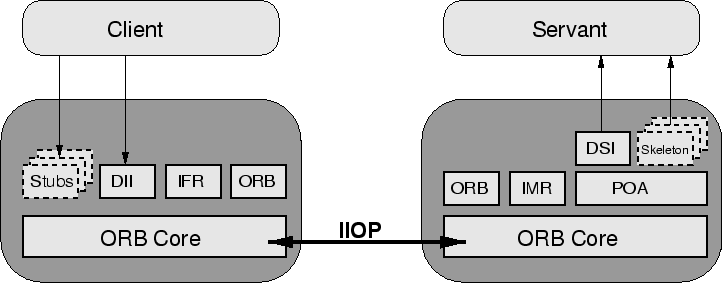
\includegraphics[width=.9\linewidth]{img/corba_archi.png}
\caption{This is the caption for the next figure link (or table)}
\end{figure}
\end{frame}
\begin{frame}[label=sec-4-14]{Transient and Persistent Objects}
Not to confound with the Persitent Object Service (POS) which allows to store object states on disk, DB,\ldots{}
\begin{block}{Transient CORBA object}
It has the same lifetime as the execution of the server process that creates it. When a server terminates, its transient objects disappear with it and any object references held by the client become invalid.
\end{block}

\begin{block}{Persistent CORBA object}
It lives until it is explicitly destroyed. If a client has a reference to it, that reference can be used even if the object’s server is not running – an ORB daemon, orbd, will start the server when the ORB receives an invocation on the object.
\end{block}
\end{frame}
\begin{frame}[label=sec-4-15]{POA}
\begin{block}{OA and POA}
\begin{itemize}
\item Object Adapter: 
mechanism that connects a request using an object reference with the proper code to service that request.

\item Portable Object Adapter: a particular type of object adapter that is 
defined by the CORBA specification.
\end{itemize}
\end{block}
\end{frame}

\begin{frame}[label=sec-4-16]{POA and Servants}
\begin{itemize}
\item A servant is the logical process that executes an object.
\item It may be mapped to one or several threads, processes, \ldots{}
\end{itemize}
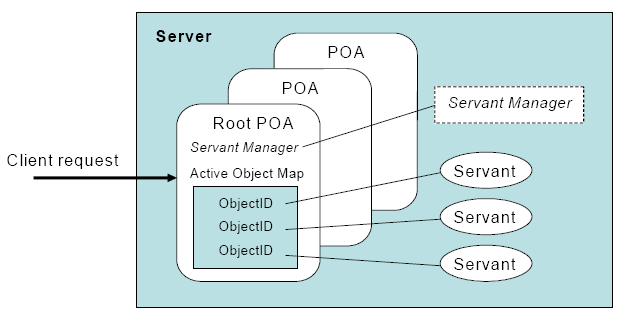
\includegraphics[width=.9\linewidth]{./img/POA.png}
\end{frame}

\begin{frame}[fragile,label=sec-4-17]{POA Control in Java (1/3)}
 \begin{block}{The first POA is managed by the ORB, and called RootPOA by convention.}
\lstset{language=java,label= ,caption= ,numbers=none}
\begin{lstlisting}
ORB orb = ORB.init( args, null );
POA rootPOA = POAHelper.narrow(
   orb.resolve_initial_references("RootPOA"));
\end{lstlisting}
\end{block}

\begin{block}{“Service” POAs can be forked from the RootPOA (it is not mandatory: you can use}
the RootPOA)
\lstset{language=java,label= ,caption= ,numbers=none}
\begin{lstlisting}
// Create a POA by passing the Persistent Policy
POA persistentPOA = rootPOA.create_POA(
      "childPOA",null,persistentPolicy );
\end{lstlisting}
\end{block}
\end{frame}

\begin{frame}[fragile,label=sec-4-18]{POA Control in Java (2/3)}
 \begin{itemize}
\item POA Manager
\end{itemize}
-- Each POA is associated a POAManager object, which starts/stops the POA, and manages the incoming requests
\lstset{language=java,label= ,caption= ,numbers=none}
\begin{lstlisting}
// If not activated, requests will hang
// because POAManager is in the 'HOLD' state.
persistentPOA.the_POAManager().activate( );
\end{lstlisting}

\begin{block}{POAManager’s States}
\begin{itemize}
\item Holding: POAs will queue incoming requests.
\item Active: POAs will start processing requests.
\item Discarding: POAs will discard incoming requests.
\item Inactive: POAs will reject the requests that have not begun executing as well as as any new requests.
\end{itemize}
\end{block}
\end{frame}


\begin{frame}[fragile,label=sec-4-19]{POA Control in Java (3/3)}
 \begin{block}{Servants}
\begin{itemize}
\item A servant may be associated
\end{itemize}
\lstset{language=java,label= ,caption= ,numbers=none}
\begin{lstlisting}
// create servant and register it with the ORB
OperationImpl o = new OperationImpl();
o.setORB(orb);
// get bject reference from the servant
org.omg.CORBA.Object ref =
      persistentPOA.servant_to_reference( o );
Operation href = OperationHelper.narrow(ref);
\end{lstlisting}
\end{block}
\end{frame}

\begin{frame}[label=sec-4-20]{POA behavior}
\begin{block}{Thread policy:}
\begin{itemize}
\item ORB$_{\text{CTRL}}$$_{\text{MODEL}}$ (default): The POA is responsible for assigning requests to threads.
\item SINGLE$_{\text{THREAD}}$$_{\text{MODEL}}$: The POA processes requests sequentially
\end{itemize}
\end{block}

\begin{block}{Lifespan policy:}
\begin{itemize}
\item TRANSIENT (Default): Objects implemented in the POA cannot outlive the process in 
which they are first created. Once the POA is deactivated, an OBJECT$_{\text{NOT}}$$_{\text{EXIST}}$ exception occurs 
when attempting to use any object references generated by the POA.
\item PERSISTENT Objects implemented in the POA can outlive the process in which they are first created.
\end{itemize}
\end{block}
\end{frame}





\begin{frame}[label=sec-4-21]{Example using Java JDK}
\begin{block}{The Sun JDK (now open-jdk) provides since a long time classes and tools to build CORBA apps.}
\end{block}
\begin{block}{Tools}
Some of the tools we will use:
\begin{itemize}
\item idlj: a compiler that maps IDL descriptions to Java
\item orbd: the Object Request Broker Daemon.
\end{itemize}
\end{block}
\end{frame}
\begin{frame}[fragile,label=sec-4-22]{NamingService (JDK): \texttt{orbd}}
 \texttt{orbd} is a name service.
\begin{itemize}
\item it allows clients to transparently locate and invoke persistent objects on servers.
\item it receives names of persistent objects from the server, and returns a reference which includes its own port (not the one of server).
\item it is persistent: if it is restarted, associations are not lost
\end{itemize}
\end{frame}

\begin{frame}[fragile,label=sec-4-23]{Example Outline}
 \begin{block}{POA Model, Transient server}
From an IDL description, we generate (\texttt{idlj}) code for a POA that starts an
Operation service as a transient server. The tasks we have to complete:
\begin{enumerate}
\item Write the IDL description of the service
\item Generates the “machinery” files with idlj
\item Write the Server code, which
\begin{itemize}
\item creates the object
\item registers the object to the POA
\item get the NamingContexExt
\item registers the object to the NamingService
\item implements the service (application code)
\end{itemize}
\item Write the Client code to test the service
\end{enumerate}
\end{block}
\end{frame}

\begin{frame}[fragile,label=sec-4-24]{The IDL for Operation}
 \lstset{language=java,label= ,caption= ,numbers=none}
\begin{lstlisting}
module SimpleComputation
{
  interface Operation
  {
  long addition(in long a, in long b);
  };
};
\end{lstlisting}

\begin{itemize}
\item Note: \emph{do not use the same names for interface and modules}
\item Generate the stubs and POA java sources:
\end{itemize}

\lstset{language=bash,label= ,caption= ,numbers=none}
\begin{lstlisting}
% idlj -f all Operation.idl
\end{lstlisting}
This creates a directory \texttt{SimpleComputation/}
\end{frame}

\begin{frame}[fragile,label=sec-4-25]{The Server for Operation}

 \end{frame}

\begin{frame}[label=sec-4-26]{The Client for Operation}
\end{frame}
\begin{frame}[fragile,label=sec-4-27]{Running the example}
 \begin{itemize}
\item Start the name server. The JDK provides \texttt{orbd}
\end{itemize}
\lstset{language=bash,label= ,caption= ,numbers=none}
\begin{lstlisting}
% orbd -ORBInitialPort 1050 &
\end{lstlisting}

\begin{itemize}
\item Start the server
\end{itemize}
\lstset{language=bash,label= ,caption= ,numbers=none}
\begin{lstlisting}
% java OperationServer -ORBInitialPort 1050 -ORBInitialHost \
   localhost

IOR: IOR:000000000000002449444c3a53696d706c65436f6d7075746174696f6e2f4f7065726174696f6e3a312e3000000000010000000000000086000102000000000d3139322e3136382e35362e310000cf3f00000031afabcb000000002083e61b0900000001000000000000000100000008526f6f74504f410000000008000000010000000014000000000000020000000100000020000000000001000100000002050100010001002000010109000000010001010000000026000000020002
OperationServer ready and waiting ...
\end{lstlisting}

\begin{itemize}
\item Start the client
\end{itemize}
\lstset{language=bash,label= ,caption= ,numbers=none}
\begin{lstlisting}
% java OperationClient -ORBInitialPort 1050 -ORBInitialHost \
  localhost
\end{lstlisting}
\end{frame}


\begin{frame}[fragile,label=sec-4-28]{\texttt{servertool} (JDK)}
 A command line tool to register, unregister, startup and shutdown a
server.

\lstset{language=bash,label= ,caption= ,numbers=none}
\begin{lstlisting}
 % servertool -ORBInitialPort 1050
 servertool > register -server OperationServer \
 -applicationName MyOp
           server registered (ID server = 0).
 servertool > list
       Server Id Server Class Name Server Application
       --------- ----------------- ------------------
       257 OperationServer MyOp
\end{lstlisting}
\end{frame}
% Emacs 24.4.51.2 (Org mode 8.2.10)
\end{document}
